\chapter{Sorting}

\index{sorting}

\key{Sorting}
is a fundamental algorithm design problem.
In addition,
many efficient algorithms
use sorting as a subroutine,
because it is often easier to process
data if the elements are in a sorted order.

For example, the question ''does the array contain
two equal elements?'' is easy to solve using sorting.
If the array contains two equal elements,
they will be next to each other after sorting,
so it is easy to find them.
Also the question ''what is the most frequent element
in the array?'' can be solved similarly.

There are many algorithms for sorting, that are
also good examples of algorithm design techniques.
The efficient general sorting algorithms
work in $O(n \log n)$ time,
and many algorithms that use sorting
as a subroutine also
have this time complexity.

\section{Sorting theory}

The basic problem in sorting is as follows:
\begin{framed}
\noindent
Given an array that contains $n$ elements,
your task is to sort the elements
in increasing order.
\end{framed}
\noindent
For example, the array
\begin{center}
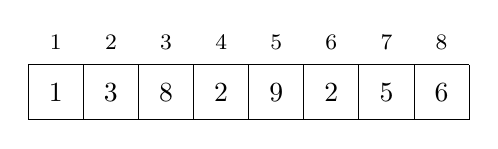
\begin{tikzpicture}[scale=0.7]
\draw (0,0) grid (8,1);
\node at (0.5,0.5) {$1$};
\node at (1.5,0.5) {$3$};
\node at (2.5,0.5) {$8$};
\node at (3.5,0.5) {$2$};
\node at (4.5,0.5) {$9$};
\node at (5.5,0.5) {$2$};
\node at (6.5,0.5) {$5$};
\node at (7.5,0.5) {$6$};

\footnotesize
\node at (0.5,1.4) {$1$};
\node at (1.5,1.4) {$2$};
\node at (2.5,1.4) {$3$};
\node at (3.5,1.4) {$4$};
\node at (4.5,1.4) {$5$};
\node at (5.5,1.4) {$6$};
\node at (6.5,1.4) {$7$};
\node at (7.5,1.4) {$8$};
\end{tikzpicture}
\end{center}
will be as follows after sorting:
\begin{center}
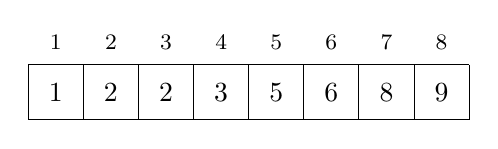
\begin{tikzpicture}[scale=0.7]
\draw (0,0) grid (8,1);
\node at (0.5,0.5) {$1$};
\node at (1.5,0.5) {$2$};
\node at (2.5,0.5) {$2$};
\node at (3.5,0.5) {$3$};
\node at (4.5,0.5) {$5$};
\node at (5.5,0.5) {$6$};
\node at (6.5,0.5) {$8$};
\node at (7.5,0.5) {$9$};

\footnotesize
\node at (0.5,1.4) {$1$};
\node at (1.5,1.4) {$2$};
\node at (2.5,1.4) {$3$};
\node at (3.5,1.4) {$4$};
\node at (4.5,1.4) {$5$};
\node at (5.5,1.4) {$6$};
\node at (6.5,1.4) {$7$};
\node at (7.5,1.4) {$8$};
\end{tikzpicture}
\end{center}

\subsubsection{$O(n^2)$ algorithms}

\index{bubble sort}

Simple algorithms for sorting an array
work in $O(n^2)$ time.
Such algorithms are short and usually
consist of two nested loops.
A famous $O(n^2)$ time algorithm for sorting
is \key{bubble sort} where the elements
''bubble'' forward in the array according to their values.

Bubble sort consists of $n-1$ rounds.
On each round, the algorithm iterates through
the elements in the array.
Whenever two successive elements are found
that are not in correct order,
the algorithm swaps them.
The algorithm can be implemented as follows
for array
$\texttt{t}[1],\texttt{t}[2],\ldots,\texttt{t}[n]$:
\begin{lstlisting}
for (int i = 1; i <= n-1; i++) {
    for (int j = 1; j <= n-i; j++) {
        if (t[j] > t[j+1]) swap(t[j],t[j+1]);
    }
}
\end{lstlisting}

After the first round of the algorithm,
the largest element is in the correct place,
after the second round the second largest
element is in the correct place, etc.
Thus, after $n-1$ rounds, all elements
will be sorted.

For example, in the array

\begin{center}
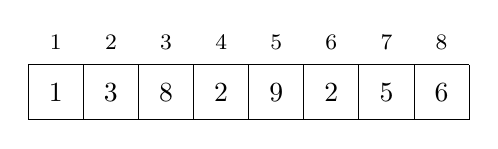
\begin{tikzpicture}[scale=0.7]
\draw (0,0) grid (8,1);

\node at (0.5,0.5) {$1$};
\node at (1.5,0.5) {$3$};
\node at (2.5,0.5) {$8$};
\node at (3.5,0.5) {$2$};
\node at (4.5,0.5) {$9$};
\node at (5.5,0.5) {$2$};
\node at (6.5,0.5) {$5$};
\node at (7.5,0.5) {$6$};

\footnotesize
\node at (0.5,1.4) {$1$};
\node at (1.5,1.4) {$2$};
\node at (2.5,1.4) {$3$};
\node at (3.5,1.4) {$4$};
\node at (4.5,1.4) {$5$};
\node at (5.5,1.4) {$6$};
\node at (6.5,1.4) {$7$};
\node at (7.5,1.4) {$8$};
\end{tikzpicture}
\end{center}

\noindent
the first round of bubble sort swaps elements
as follows:

\begin{center}
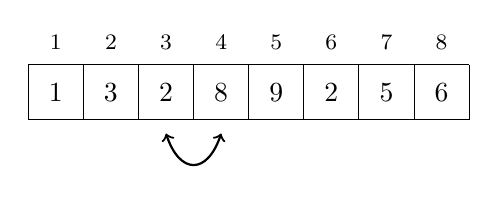
\begin{tikzpicture}[scale=0.7]
\draw (0,0) grid (8,1);
\node at (0.5,0.5) {$1$};
\node at (1.5,0.5) {$3$};
\node at (2.5,0.5) {$2$};
\node at (3.5,0.5) {$8$};
\node at (4.5,0.5) {$9$};
\node at (5.5,0.5) {$2$};
\node at (6.5,0.5) {$5$};
\node at (7.5,0.5) {$6$};

\draw[thick,<->] (3.5,-0.25) .. controls (3.25,-1.00) and (2.75,-1.00) .. (2.5,-0.25);

\footnotesize
\node at (0.5,1.4) {$1$};
\node at (1.5,1.4) {$2$};
\node at (2.5,1.4) {$3$};
\node at (3.5,1.4) {$4$};
\node at (4.5,1.4) {$5$};
\node at (5.5,1.4) {$6$};
\node at (6.5,1.4) {$7$};
\node at (7.5,1.4) {$8$};
\end{tikzpicture}
\end{center}

\begin{center}
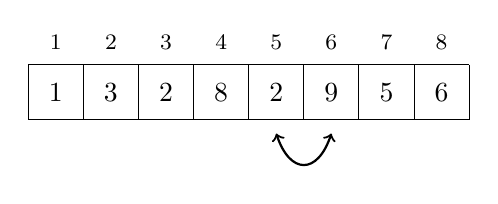
\begin{tikzpicture}[scale=0.7]
\draw (0,0) grid (8,1);
\node at (0.5,0.5) {$1$};
\node at (1.5,0.5) {$3$};
\node at (2.5,0.5) {$2$};
\node at (3.5,0.5) {$8$};
\node at (4.5,0.5) {$2$};
\node at (5.5,0.5) {$9$};
\node at (6.5,0.5) {$5$};
\node at (7.5,0.5) {$6$};

\draw[thick,<->] (5.5,-0.25) .. controls (5.25,-1.00) and (4.75,-1.00) .. (4.5,-0.25);


\footnotesize
\node at (0.5,1.4) {$1$};
\node at (1.5,1.4) {$2$};
\node at (2.5,1.4) {$3$};
\node at (3.5,1.4) {$4$};
\node at (4.5,1.4) {$5$};
\node at (5.5,1.4) {$6$};
\node at (6.5,1.4) {$7$};
\node at (7.5,1.4) {$8$};
\end{tikzpicture}
\end{center}

\begin{center}
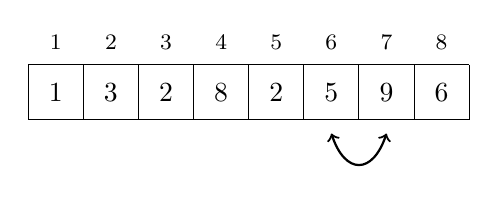
\begin{tikzpicture}[scale=0.7]
\draw (0,0) grid (8,1);
\node at (0.5,0.5) {$1$};
\node at (1.5,0.5) {$3$};
\node at (2.5,0.5) {$2$};
\node at (3.5,0.5) {$8$};
\node at (4.5,0.5) {$2$};
\node at (5.5,0.5) {$5$};
\node at (6.5,0.5) {$9$};
\node at (7.5,0.5) {$6$};

\draw[thick,<->] (6.5,-0.25) .. controls (6.25,-1.00) and (5.75,-1.00) .. (5.5,-0.25);


\footnotesize
\node at (0.5,1.4) {$1$};
\node at (1.5,1.4) {$2$};
\node at (2.5,1.4) {$3$};
\node at (3.5,1.4) {$4$};
\node at (4.5,1.4) {$5$};
\node at (5.5,1.4) {$6$};
\node at (6.5,1.4) {$7$};
\node at (7.5,1.4) {$8$};
\end{tikzpicture}
\end{center}

\begin{center}
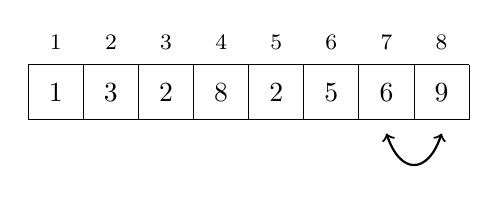
\begin{tikzpicture}[scale=0.7]
\draw (0,0) grid (8,1);
\node at (0.5,0.5) {$1$};
\node at (1.5,0.5) {$3$};
\node at (2.5,0.5) {$2$};
\node at (3.5,0.5) {$8$};
\node at (4.5,0.5) {$2$};
\node at (5.5,0.5) {$5$};
\node at (6.5,0.5) {$6$};
\node at (7.5,0.5) {$9$};

\draw[thick,<->] (7.5,-0.25) .. controls (7.25,-1.00) and (6.75,-1.00) .. (6.5,-0.25);

\footnotesize
\node at (0.5,1.4) {$1$};
\node at (1.5,1.4) {$2$};
\node at (2.5,1.4) {$3$};
\node at (3.5,1.4) {$4$};
\node at (4.5,1.4) {$5$};
\node at (5.5,1.4) {$6$};
\node at (6.5,1.4) {$7$};
\node at (7.5,1.4) {$8$};
\end{tikzpicture}
\end{center}

\subsubsection{Inversions}

\index{inversion}

Bubble sort is an example of a sorting
algorithm that always swaps successive
elements in the array.
It turns out that the time complexity
of this kind of an algorithm is \emph{always}
at least $O(n^2)$ because in the worst case,
$O(n^2)$ swaps are required for sorting the array.

A useful concept when analyzing sorting
algorithms is an \key{inversion}.
It is a pair of elements
$(\texttt{t}[a],\texttt{t}[b])$
in the array such that
$a<b$ and $\texttt{t}[a]>\texttt{t}[b]$,
i.e., they are in wrong order.
For example, in the array
\begin{center}
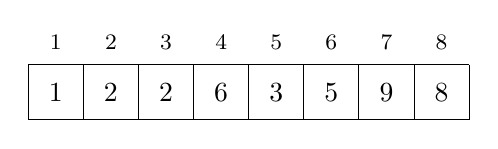
\begin{tikzpicture}[scale=0.7]
\draw (0,0) grid (8,1);
\node at (0.5,0.5) {$1$};
\node at (1.5,0.5) {$2$};
\node at (2.5,0.5) {$2$};
\node at (3.5,0.5) {$6$};
\node at (4.5,0.5) {$3$};
\node at (5.5,0.5) {$5$};
\node at (6.5,0.5) {$9$};
\node at (7.5,0.5) {$8$};

\footnotesize
\node at (0.5,1.4) {$1$};
\node at (1.5,1.4) {$2$};
\node at (2.5,1.4) {$3$};
\node at (3.5,1.4) {$4$};
\node at (4.5,1.4) {$5$};
\node at (5.5,1.4) {$6$};
\node at (6.5,1.4) {$7$};
\node at (7.5,1.4) {$8$};
\end{tikzpicture}
\end{center}
the inversions are $(6,3)$, $(6,5)$ and $(9,8)$.
The number of inversions indicates
how sorted the array is.
An array is completely sorted when
there are no inversions.
On the other hand, if the array elements
are in reverse order,
the number of inversions is maximum:
\[1+2+\cdots+(n-1)=\frac{n(n-1)}{2} = O(n^2)\]

Swapping successive elements that are
in wrong order removes exactly one inversion
from the array.
Thus, if a sorting algorithm can only
swap successive elements, each swap removes
at most one inversion and the time complexity
of the algorithm is at least $O(n^2)$.

\subsubsection{$O(n \log n)$ algorithms}

\index{merge sort}

It is possible to sort an array efficiently
in $O(n \log n)$ time using an algorithm
that is not limited to swapping successive elements.
One such algorithm is \key{mergesort}
that sorts an array recursively by dividing
it into smaller subarrays.

Mergesort sorts the subarray $[a,b]$ as follows:

\begin{enumerate}
\item If $a=b$, don't do anything because the subarray is already sorted.
\item Calculate the index of the middle element: $k=\lfloor (a+b)/2 \rfloor$.
\item Recursively sort the subarray $[a,k]$.
\item Recursively sort the subarray $[k+1,b]$.
\item \emph{Merge} the sorted subarrays $[a,k]$ and $[k+1,b]$
into a sorted subarray $[a,b]$.
\end{enumerate}

Mergesort is an efficient algorithm because it
halves the size of the subarray at each step.
The recursion consists of $O(\log n)$ levels,
and processing each level takes $O(n)$ time.
Merging the subarrays $[a,k]$ and $[k+1,b]$
is possible in linear time because they are already sorted.

For example, consider sorting the following array:
\begin{center}
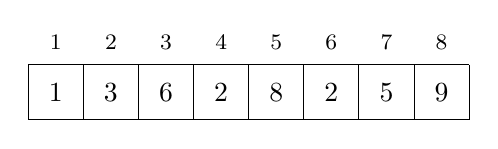
\begin{tikzpicture}[scale=0.7]
\draw (0,0) grid (8,1);
\node at (0.5,0.5) {$1$};
\node at (1.5,0.5) {$3$};
\node at (2.5,0.5) {$6$};
\node at (3.5,0.5) {$2$};
\node at (4.5,0.5) {$8$};
\node at (5.5,0.5) {$2$};
\node at (6.5,0.5) {$5$};
\node at (7.5,0.5) {$9$};

\footnotesize
\node at (0.5,1.4) {$1$};
\node at (1.5,1.4) {$2$};
\node at (2.5,1.4) {$3$};
\node at (3.5,1.4) {$4$};
\node at (4.5,1.4) {$5$};
\node at (5.5,1.4) {$6$};
\node at (6.5,1.4) {$7$};
\node at (7.5,1.4) {$8$};
\end{tikzpicture}
\end{center}

The array will be divided into two subarrays
as follows:
\begin{center}
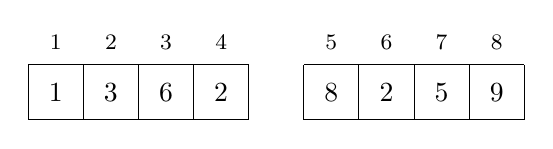
\begin{tikzpicture}[scale=0.7]
\draw (0,0) grid (4,1);
\draw (5,0) grid (9,1);

\node at (0.5,0.5) {$1$};
\node at (1.5,0.5) {$3$};
\node at (2.5,0.5) {$6$};
\node at (3.5,0.5) {$2$};

\node at (5.5,0.5) {$8$};
\node at (6.5,0.5) {$2$};
\node at (7.5,0.5) {$5$};
\node at (8.5,0.5) {$9$};

\footnotesize
\node at (0.5,1.4) {$1$};
\node at (1.5,1.4) {$2$};
\node at (2.5,1.4) {$3$};
\node at (3.5,1.4) {$4$};
\node at (5.5,1.4) {$5$};
\node at (6.5,1.4) {$6$};
\node at (7.5,1.4) {$7$};
\node at (8.5,1.4) {$8$};

\end{tikzpicture}
\end{center}

Then, the subarrays will be sorted recursively
as follows:
\begin{center}
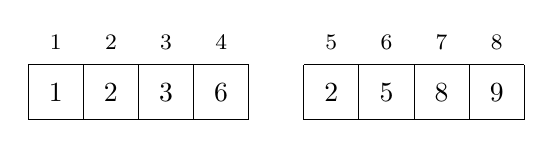
\begin{tikzpicture}[scale=0.7]
\draw (0,0) grid (4,1);
\draw (5,0) grid (9,1);

\node at (0.5,0.5) {$1$};
\node at (1.5,0.5) {$2$};
\node at (2.5,0.5) {$3$};
\node at (3.5,0.5) {$6$};

\node at (5.5,0.5) {$2$};
\node at (6.5,0.5) {$5$};
\node at (7.5,0.5) {$8$};
\node at (8.5,0.5) {$9$};

\footnotesize
\node at (0.5,1.4) {$1$};
\node at (1.5,1.4) {$2$};
\node at (2.5,1.4) {$3$};
\node at (3.5,1.4) {$4$};
\node at (5.5,1.4) {$5$};
\node at (6.5,1.4) {$6$};
\node at (7.5,1.4) {$7$};
\node at (8.5,1.4) {$8$};
\end{tikzpicture}
\end{center}

Finally, the algorithm merges the sorted
subarrays and creates the final sorted array:
\begin{center}
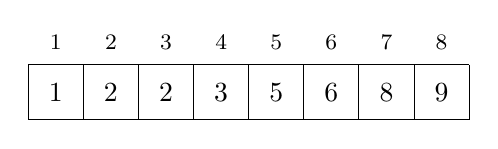
\begin{tikzpicture}[scale=0.7]
\draw (0,0) grid (8,1);
\node at (0.5,0.5) {$1$};
\node at (1.5,0.5) {$2$};
\node at (2.5,0.5) {$2$};
\node at (3.5,0.5) {$3$};
\node at (4.5,0.5) {$5$};
\node at (5.5,0.5) {$6$};
\node at (6.5,0.5) {$8$};
\node at (7.5,0.5) {$9$};

\footnotesize
\node at (0.5,1.4) {$1$};
\node at (1.5,1.4) {$2$};
\node at (2.5,1.4) {$3$};
\node at (3.5,1.4) {$4$};
\node at (4.5,1.4) {$5$};
\node at (5.5,1.4) {$6$};
\node at (6.5,1.4) {$7$};
\node at (7.5,1.4) {$8$};
\end{tikzpicture}
\end{center}

\subsubsection{Sorting lower bound}

Is it possible to sort an array faster
than in $O(n \log n)$ time?
It turns out that this is \emph{not} possible
when we restrict ourselves to sorting algorithms
that are based on comparing array elements.

The lower bound for the time complexity
can be proved by examining the sorting
as a process where each comparison of two elements
gives more information about the contents of the array.
The process creates the following tree:

\begin{center}
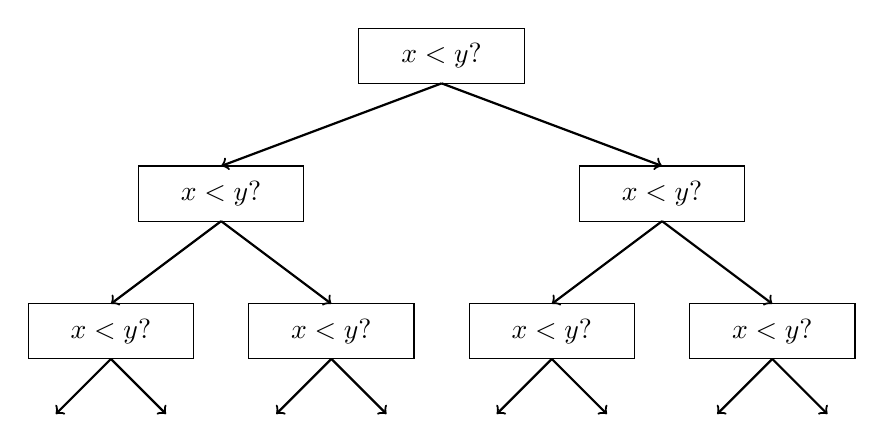
\begin{tikzpicture}[scale=0.7]
\draw (0,0) rectangle (3,1);
\node at (1.5,0.5) {$x < y?$};

\draw[thick,->] (1.5,0) -- (-2.5,-1.5);
\draw[thick,->] (1.5,0) -- (5.5,-1.5);

\draw (-4,-2.5) rectangle (-1,-1.5);
\draw (4,-2.5) rectangle (7,-1.5);
\node at (-2.5,-2) {$x < y?$};
\node at (5.5,-2) {$x < y?$};

\draw[thick,->] (-2.5,-2.5) -- (-4.5,-4);
\draw[thick,->] (-2.5,-2.5) -- (-0.5,-4);
\draw[thick,->] (5.5,-2.5) -- (3.5,-4);
\draw[thick,->] (5.5,-2.5) -- (7.5,-4);

\draw (-6,-5) rectangle (-3,-4);
\draw (-2,-5) rectangle (1,-4);
\draw (2,-5) rectangle (5,-4);
\draw (6,-5) rectangle (9,-4);
\node at (-4.5,-4.5) {$x < y?$};
\node at (-0.5,-4.5) {$x < y?$};
\node at (3.5,-4.5) {$x < y?$};
\node at (7.5,-4.5) {$x < y?$};

\draw[thick,->] (-4.5,-5) -- (-5.5,-6);
\draw[thick,->] (-4.5,-5) -- (-3.5,-6);
\draw[thick,->] (-0.5,-5) -- (0.5,-6);
\draw[thick,->] (-0.5,-5) -- (-1.5,-6);
\draw[thick,->] (3.5,-5) -- (2.5,-6);
\draw[thick,->] (3.5,-5) -- (4.5,-6);
\draw[thick,->] (7.5,-5) -- (6.5,-6);
\draw[thick,->] (7.5,-5) -- (8.5,-6);
\end{tikzpicture}
\end{center}

Here ''$x<y?$'' means that some elements
$x$ and $y$ are compared.
If $x<y$, the process continues to the left,
and otherwise to the right.
The results of the process are the possible
ways to order the array, a total of $n!$ ways.
For this reason, the height of the tree
must be at least
\[ \log_2(n!) = \log_2(1)+\log_2(2)+\cdots+\log_2(n).\]
We get an lower bound for this sum
by choosing last $n/2$ elements and
changing the value of each element to $\log_2(n/2)$.
This yields an estimate
\[ \log_2(n!) \ge (n/2) \cdot \log_2(n/2),\]
so the height of the tree and the minimum
possible number of steps in an sorting
algorithm in the worst case
is at least $n \log n$.

\subsubsection{Counting sort}

\index{counting sort}

The lower bound $n \log n$ doesn't apply to
algorithms that do not compare array elements
but use some other information.
An example of such an algorithm is
\key{counting sort} that sorts an array in
$O(n)$ time assuming that every element in the array
is an integer between $0 \ldots c$ where $c$
is a small constant.

The algorithm creates a \emph{bookkeeping} array
whose indices are elements in the original array.
The algorithm iterates through the original array
and calculates how many times each element
appears in the array.

For example, the array
\begin{center}
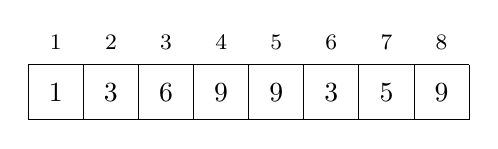
\begin{tikzpicture}[scale=0.7]
\draw (0,0) grid (8,1);
\node at (0.5,0.5) {$1$};
\node at (1.5,0.5) {$3$};
\node at (2.5,0.5) {$6$};
\node at (3.5,0.5) {$9$};
\node at (4.5,0.5) {$9$};
\node at (5.5,0.5) {$3$};
\node at (6.5,0.5) {$5$};
\node at (7.5,0.5) {$9$};

\footnotesize
\node at (0.5,1.4) {$1$};
\node at (1.5,1.4) {$2$};
\node at (2.5,1.4) {$3$};
\node at (3.5,1.4) {$4$};
\node at (4.5,1.4) {$5$};
\node at (5.5,1.4) {$6$};
\node at (6.5,1.4) {$7$};
\node at (7.5,1.4) {$8$};
\end{tikzpicture}
\end{center}
produces the following bookkeeping array:
\begin{center}
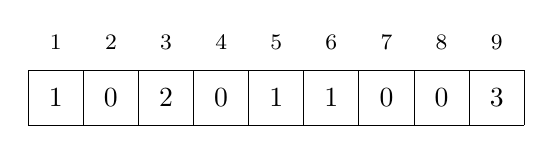
\begin{tikzpicture}[scale=0.7]
\draw (0,0) grid (9,1);
\node at (0.5,0.5) {$1$};
\node at (1.5,0.5) {$0$};
\node at (2.5,0.5) {$2$};
\node at (3.5,0.5) {$0$};
\node at (4.5,0.5) {$1$};
\node at (5.5,0.5) {$1$};
\node at (6.5,0.5) {$0$};
\node at (7.5,0.5) {$0$};
\node at (8.5,0.5) {$3$};

\footnotesize

\node at (0.5,1.5) {$1$};
\node at (1.5,1.5) {$2$};
\node at (2.5,1.5) {$3$};
\node at (3.5,1.5) {$4$};
\node at (4.5,1.5) {$5$};
\node at (5.5,1.5) {$6$};
\node at (6.5,1.5) {$7$};
\node at (7.5,1.5) {$8$};
\node at (8.5,1.5) {$9$};
\end{tikzpicture}
\end{center}

For example, the value of element 3
in the bookkeeping array is 2,
because the element 3 appears two times
in the original array (indices 2 and 6).

The construction of the bookkeeping array
takes $O(n)$ time. After this, the sorted array
can be created in $O(n)$ time because
the amount of each element can be retrieved
from the bookkeeping array.
Thus, the total time complexity of counting
sort is $O(n)$.

Counting sort is a very efficient algorithm
but it can only be used when the constant $c$
is so small that the array elements can
be used as indices in the bookkeeping array.

\section{Järjestäminen C++:ssa}

\index{sort@\texttt{sort}}

Järjestämisalgoritmia
ei yleensä koskaan kannata koodata itse,
vaan on parempi ratkaisu käyttää
ohjelmointikielen valmista toteutusta.
Esimerkiksi
C++:n standardikirjastossa on funktio \texttt{sort},
jonka avulla voi järjestää helposti taulukoita
ja muita tietorakenteita.

Valmiin toteutuksen käyttämisessä on monia etuja.
Ensinnäkin se säästää aikaa, koska järjestämisalgoritmia
ei tarvitse kirjoittaa itse.
Lisäksi valmis toteutus on varmasti tehokas ja toimiva:
vaikka järjestämisalgoritmin toteuttaisi itse,
siitä tulisi tuskin valmista toteutusta parempi.

Tutustumme seuraavaksi C++:n \texttt{sort}-funktion
käyttämiseen.
Seuraava koodi järjestää vektorin \texttt{v}
luvut pienimmästä suurimpaan:
\begin{lstlisting}
vector<int> v = {4,2,5,3,5,8,3};
sort(v.begin(),v.end());
\end{lstlisting}
Järjestämisen seurauksena
vektorin sisällöksi tulee
$\{2,3,3,4,5,5,8\}$.
Oletuksena \texttt{sort}-funktio järjestää
siis alkiot pienimmästä suurimpaan,
mutta järjestyksen saa käänteiseksi näin:
\begin{lstlisting}
sort(v.rbegin(),v.rend());
\end{lstlisting}
Tavallisen taulukon voi järjestää seuraavasti:
\begin{lstlisting}
int n = 7; // taulukon koko
int t[] = {4,2,5,3,5,8,3};
sort(t,t+n);
\end{lstlisting}
Seuraava koodi taas järjestää merkkijonon \texttt{s}:
\begin{lstlisting}
string s = "apina";
sort(s.begin(), s.end());
\end{lstlisting}
Merkkijonon järjestäminen tarkoittaa,
että sen merkit järjestetään aakkosjärjestykseen.
Esimerkiksi merkkijono ''apina''
on järjestettynä ''aainp''.

\subsubsection{Vertailuoperaattori}

\index{vertailuoperaattori@vertailuoperaattori}

Funktion \texttt{sort} käyttäminen vaatii,
että järjestettävien alkioiden
tietotyypille on määritelty \key{vertailuoperaattori} \texttt{<},
jonka avulla voi selvittää, mikä on kahden alkion järjestys.
Järjestämisen aikana \texttt{sort}-funktio
käyttää operaattoria \texttt{<} aina, kun sen täytyy
vertailla järjestettäviä alkioita.

Vertailuoperaattori on määritelty valmiiksi
useimmille C++:n tietotyypeille,
minkä ansiosta niitä pystyy järjestämään automaattisesti.
Jos järjestettävänä on lukuja, ne järjestyvät
suuruusjärjestykseen,
ja jos järjestettävänä on merkkijonoja,
ne järjestyvät aakkosjärjestykseen.

\index{pair@\texttt{pair}}

Parit (\texttt{pair}) järjestyvät ensisijaisesti
ensimmäisen kentän (\texttt{first}) mukaan.
Jos kuitenkin parien ensimmäiset kentät ovat samat,
järjestys määräytyy toisen kentän (\texttt{second}) mukaan:
\begin{lstlisting}
vector<pair<int,int>> v;
v.push_back({1,5});
v.push_back({2,3});
v.push_back({1,2});
sort(v.begin(), v.end());
\end{lstlisting}
Tämän seurauksena parien järjestys on
$(1,2)$, $(1,5)$ ja $(2,3)$.

\index{tuple@\texttt{tuple}}
Vastaavasti \texttt{tuple}-rakenteet
järjestyvät ensisijaisesti ensimmäisen kentän,
toissijaisesti toisen kentän, jne., mukaan:
\begin{lstlisting}
vector<tuple<int,int,int>> v;
v.push_back(make_tuple(2,1,4));
v.push_back(make_tuple(1,5,3));
v.push_back(make_tuple(2,1,3));
sort(v.begin(), v.end());
\end{lstlisting}
Tämän seurauksena järjestys on
$(1,5,3)$, $(2,1,3)$ ja $(2,1,4)$.

\subsubsection{Omat tietueet}

Jos järjestettävänä on omia tietueita,
niiden vertailuoperaattori täytyy toteuttaa itse.
Operaattori määritellään tietueen sisään
\texttt{operator<}-nimisenä funktiona,
jonka parametrina on toinen alkio.
Operaattorin tulee palauttaa \texttt{true},
jos oma alkio on pienempi kuin parametrialkio,
ja muuten \texttt{false}.

Esimerkiksi seuraava tietue \texttt{P}
sisältää pisteen x- ja y-koordinaatit.
Vertailuoperaattori on toteutettu niin,
että pisteet järjestyvät ensisijaisesti x-koor\-di\-naa\-tin
ja toissijaisesti y-koordinaatin mukaan.

\begin{lstlisting}
struct P {
    int x, y;
    bool operator<(const P &p) {
        if (x != p.x) return x < p.x;
        else return y < p.y;
    }
};
\end{lstlisting}

\subsubsection{Vertailufunktio}

\index{vertailufunktio@vertailufunktio}

On myös mahdollista antaa
\texttt{sort}-funktiolle ulkopuolinen \key{vertailufunktio}.
Esimerkiksi seuraava vertailufunktio
järjestää merkkijonot ensisijaisesti pituuden mukaan
ja toissijaisesti aakkosjärjestyksen mukaan:

\begin{lstlisting}
bool cmp(string a, string b) {
    if (a.size() != b.size()) return a.size() < b.size();
    return a < b;
}
\end{lstlisting}
Tämän jälkeen merkkijonovektorin voi järjestää näin:
\begin{lstlisting}
sort(v.begin(), v.end(), cmp);
\end{lstlisting}

\section{Binäärihaku}

\index{binxxrihaku@binäärihaku}

Tavallinen tapa etsiä alkiota taulukosta
on käyttää \texttt{for}-silmukkaa, joka käy läpi
taulukon sisällön alusta loppuun.
Esimerkiksi seuraava koodi etsii alkiota
$x$ taulukosta \texttt{t}.

\begin{lstlisting}
for (int i = 1; i <= n; i++) {
    if (t[i] == x) // alkio x löytyi kohdasta i
}
\end{lstlisting}

Tämän menetelmän aikavaativuus on $O(n)$,
koska pahimmassa tapauksessa koko taulukko täytyy
käydä läpi.
Jos taulukon sisältö voi olla mikä tahansa,
tämä on kuitenkin tehokkain mahdollinen menetelmä,
koska saatavilla ei ole lisätietoa siitä,
mistä päin taulukkoa alkiota $x$ kannattaa etsiä.

Tilanne on toinen silloin, kun taulukko on
järjestyksessä.
Tässä tapauksessa haku on mahdollista toteuttaa
paljon nopeammin, koska taulukon järjestys
ohjaa etsimään alkiota oikeasta suunnasta.
Seuraavaksi käsiteltävä \key{binäärihaku}
löytää alkion järjestetystä taulukosta
tehokkaasti ajassa $O(\log n)$.

\subsubsection{Toteutus 1}

Perinteinen tapa toteuttaa binäärihaku muistuttaa sanan etsimistä
sanakirjasta. Haku puolittaa joka askeleella hakualueen taulukossa,
kunnes lopulta etsittävä alkio löytyy tai osoittautuu,
että sitä ei ole taulukossa.

Haku tarkistaa ensin taulukon keskimmäisen alkion.
Jos keskimmäinen alkio on etsittävä alkio, haku päättyy.
Muuten haku jatkuu taulukon vasempaan tai oikeaan osaan sen mukaan,
onko keskimmäinen alkio suurempi vain pienempi kuin etsittävä alkio.

Yllä olevan idean voi toteuttaa seuraavasti:
\begin{lstlisting}
int a = 1, b = n;
while (a <= b) {
    int k = (a+b)/2;
    if (t[k] == x) // alkio x löytyi kohdasta k
    if (t[k] > x) b = k-1;
    else a = k+1;
}
\end{lstlisting}

Algoritmi pitää yllä väliä $a \ldots b$, joka on
jäljellä oleva hakualue taulukossa.
Aluksi väli on $1 \ldots n$ eli koko taulukko.
Välin koko puolittuu algoritmin joka vaiheessa,
joten aikavaativuus on $O(\log n)$.

\subsubsection{Toteutus 2}

Vaihtoehtoinen tapa toteuttaa binäärihaku
perustuu taulukon tehostettuun läpikäyntiin.
Ideana on käydä taulukkoa läpi hyppien
ja hidastaa vauhtia, kun etsittävä alkio lähestyy.

Haku käy taulukkoa läpi vasemmalta oikealle aloittaen
hypyn pituudesta $n/2$.
Joka vaiheessa hypyn pituus puolittuu:
ensin $n/4$, sitten $n/8$, sitten $n/16$ jne.,
kunnes lopulta hypyn pituus on 1.
Hyppyjen jälkeen joko haettava alkio on löytynyt
tai selviää, että sitä ei ole taulukossa.

Seuraava koodi toteuttaa äskeisen idean:
\begin{lstlisting}
int k = 1;
for (int b = n/2; b >= 1; b /= 2) {
    while (k+b <= n && t[k+b] <= x) k += b;
}
if (t[k] == x) // alkio x löytyi kohdasta k
\end{lstlisting}

Muuttuja $k$ on läpikäynnin kohta taulukossa
ja muuttuja $b$ on hypyn pituus.
Jos alkio $x$ esiintyy taulukossa,
sen kohta on muuttujassa $k$ algoritmin päätteeksi.
Algoritmin aikavaativuus on $O(\log n)$,
koska \texttt{while}-silmukassa oleva koodi suoritetaan
aina enintään kahdesti.

\subsubsection{Muutoskohdan etsiminen}

Käytännössä binäärihakua tarvitsee toteuttaa
harvoin alkion etsimiseen taulukosta,
koska sen sijasta voi käyttää standardikirjastoa.
Esimerkiksi C++:n funktiot \texttt{lower\_bound}
ja \texttt{upper\_bound} toteuttavat binäärihaun
ja tietorakenne \texttt{set} ylläpitää joukkoa,
jonka operaatiot ovat $O(\log n)$-aikaisia.

Sitäkin tärkeämpi binäärihaun käyttökohde on 
funktion \key{muutoskohdan} etsiminen.
Oletetaan, että haluamme löytää pienimmän arvon $k$,
joka on kelvollinen ratkaisu ongelmaan.
Käytössämme on funktio $\texttt{ok}(x)$,
joka palauttaa \texttt{true}, jos $x$ on kelvollinen
ratkaisu, ja muuten \texttt{false}.
Lisäksi tiedämme, että $\texttt{ok}(x)$ on \texttt{false}
aina kun $x<k$ ja \texttt{true} aina kun $x \geq k$.
% Toisin sanoen haluamme löytää funktion \texttt{ok} \emph{muutoskohdan},
% jossa arvosta \texttt{false} tulee arvo \texttt{true}.
Tilanne näyttää seuraavalta:

\begin{center}
\begin{tabular}{r|rrrrrrrr}
$x$ & 0 & 1 & $\cdots$ & $k-1$ & $k$ & $k+1$ & $\cdots$ \\
\hline
$\texttt{ok}(x)$ & \texttt{false} & \texttt{false}
& $\cdots$ & \texttt{false} & \texttt{true} & \texttt{true} & $\cdots$ \\
\end{tabular}
\end{center}

\noindent
Nyt muutoskohta on mahdollista etsiä käyttämällä
binäärihakua:

\begin{lstlisting}
int x = -1;
for (int b = z; b >= 1; b /= 2) {
    while (!ok(x+b)) x += b;
}
int k = x+1;
\end{lstlisting}

Haku etsii suurimman $x$:n arvon,
jolla $\texttt{ok}(x)$ on \texttt{false}.
Niinpä tästä seuraava arvo $k=x+1$
on pienin arvo, jolla $\texttt{ok}(k)$ on \texttt{true}.
Hypyn aloituspituus $z$ tulee olla 
sopiva suuri luku, esimerkiksi sellainen,
jolla $\texttt{ok}(z)$ on varmasti \texttt{true}.

Algoritmi kutsuu $O(\log z)$ kertaa funktiota
\texttt{ok}, joten kokonaisaikavaativuus
riippuu siitä, kauanko funktion \texttt{ok}
suoritus kestää.
Esimerkiksi jos ratkaisun tarkastus
vie aikaa $O(n)$, niin kokonaisaikavaativuus
on $O(n \log z)$.

\subsubsection{Huippuarvon etsiminen}

Binäärihaulla voi myös etsiä
suurimman arvon funktiolle,
joka on ensin kasvava ja sitten laskeva.
Toisin sanoen tehtävänä on etsiä arvo
$k$ niin, että

\begin{itemize}
\item
$f(x)<f(x+1)$, kun $x<k$, ja
\item
$f(x)>f(x+1)$, kun $x >= k$.
\end{itemize}

Ideana on etsiä binäärihaulla
viimeinen kohta $x$,
jossa pätee $f(x)<f(x+1)$.
Tällöin $k=x+1$,
koska pätee $f(x+1)>f(x+2)$.
Seuraava koodi toteuttaa haun: 

\begin{lstlisting}
int x = -1;
for (int b = z; b >= 1; b /= 2) {
    while (f(x+b) < f(x+b+1)) x += b;
}
int k = x+1;
\end{lstlisting}

Huomaa, että toisin kuin tavallisessa binäärihaussa,
tässä ei ole sallittua,
että peräkkäiset arvot olisivat yhtä suuria.
Silloin ei olisi mahdollista tietää,
mihin suuntaan hakua tulee jatkaa.



